\newpage

\begin{itemize}

\section{DOMANDE}

\item scelte progettuali a livello di architettura: perché e quali?

In base all'analisi dei requisiti e del problema, si è pensato di 
    - realizzare un sistema distribuito (console e robot, le diverse parti che girano su nodi diversi) e eterogeneo (sistemi qakactor, node). per permettere alle varie parti di comunicare si utilizzano un modello basato su messaggi e eventi ( qkactor: dipsatch e event -> attore kotlin: coda di messaggi)
    - usare un'architettura esagonale (modello tipico dell'IoT), modello delle risorse al centro. tutte le modifiche al sistema sono precedute da una modifica al modello delle risorse (es. model change inviati a resourcemodel, resource model li manda a robotmind). 

\item  Collegare le scelte progettuali ai principi studiati durante il corso (model driven development, "non c'é codice senza progetto", le fasi Scrum, la software factory ecc).

model driven development (a mano o automatizzato)-> è modalità di sviluppo software, cambio modello -> cambia codice \\
software factory -> tool con metalinguaggio che genera codice 
non c'è codice senza progetto, non c'è progetto senza analisi del problema, non c'è analisi del problema senza analisi dei requisiti -> abbiamo usato questo approccio nel codice e nella rel\\
fasi scrum -> scrum è metodologie Agile. È  definita da Ruoli (product owner, scrum master, team di sviluppo), Artefatti (Product Backlog - inizio -, Sprint Backlog - ogni sprint, e Incremento) ed Eventi (Sprint Planning, Daily Scrum, Sprint Review, Sprint Review, Retrospective).\\
 
\item Qual è la differenza tra analisi dei requisiti e analisi del problema? 
analisi dei requisiti -> COSA
analisi del problema -> COME, problematiche

(la differenza non è marcata da una linea netta ma suscettibile di varie interpretazioni e spiegare)

\item Qual è l’architettura logica del sistema? 
foglio stampato 

\item Da quante parti è composto il vostro sistema?

2 contesti (nodi) + 1 console in remoto 

\item Spiegare perché avete evocato un certo concetto in una fase piuttosto che nell'altra?
(l'importante in questo caso è avere le idee chiare e saper fornire un ragionamento logico)

\item Qual è il rapporto (quindi interazione) tra i componenti del sistema?

messaggi e eventi: fra web server e  contesto della mind (eventi sparati sulla topic qak/events, messaggi inviati sulla topic del qkactor)
messaggi: da contesto della mind a contesto actuator
	
\item Che modello delle risorse avete usato? Come funziona?
informazioni sullo stato robot 

Nel nostro progetto il modello delle risorse è gestito mediante le plannerUtils. In particolare:

Rombo pieno = composizione (persona, cuore -> la persona non eistenza senza cuore)
rombo vuoto = aggregazione (casa, divano -> la casa esiste anche senza divano)

Per rendere le risorse accessibili via web abbiamo utilizzato CoAP (il resourcemodel manda updatemodel(che emette evento modelContent (MQTT) e aggiorno risorsa CoAP)).

\begin{figure} [H]
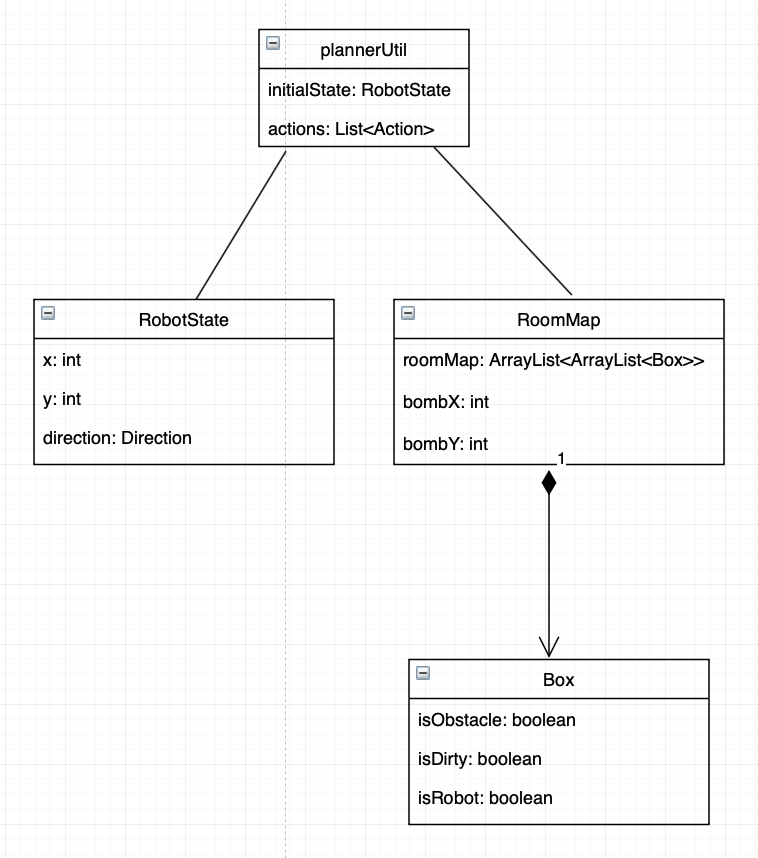
\includegraphics[width=\linewidth]{img/modello_risorse_java.png}
\end{figure}


\item Come avete fatto la rappresentazione della base di  conoscenza?

- inizio, prolog -> rappresentavamo solo stato del robot \\
- poi, tolto prolog -> abbiamo usato le plannerUtils -> rappresentavamo stato del robot, mappa e bagaglio
(non dire: la temperatura non la salviamo nelle plannerUtils)

\item Problema della consistenza: come mantenete la consistenza tra modelli delle risorse diversi?


Unico modello delle risorse (gestito in PlannerUtils).\\

consistenza tra PlannerUtils e CoAP.\\

ogni volta che cambiamo qualcosa nelle PlannerUtils, l'attore resourceModel aggiorna la risorsa CoAP (non dire: di fatto lo fa mandando un modelContent a MQTT)\\

\item Come è gestita l’interazione tra i diversi attori? 

riguardare i messaggi che si scambiano tra attori 

\item Il framework dei qactor è message based/driven, event based/driven?

message based, event based/driven

\item test plan: cosa sono e quando vanno fatti?
servono a verificare la correttezza del sistema in maniera automatzzata.
(posso sia implementarli prima di fare l'imple o anche dopo, se prima -> non funzioneranno)

\item Struttura, comportamento e interazione per ogni componente del sistema?

\item Struttura, comportamento e interazione per il sistema?
Struttura del sistema su quale nodo (contesto) mi trovo,
comportamento degli attori, 
interazione -> comunicazione con messaggi e eventi nel sistema

\item Come usate MQTT? Perché avete usato MQTT? E non, ad esempio, TCP?
MQTT per gestire scambio di messaggi (eventi gestiti sulla topic come messaggi), usa patter publish/subscribe e fornisce delle astrazioni più ad alto livello. 

\item Come usate CoAP? Perché avete usato CoAP?

rendere disp. via web. le info del nostro sistema. CoAP è : implementazione del protocollo restfull + usato in ambito iot.

\item Quali sono le parti del vostro sistema fisico?

-l'applicazione web\\
-l'applicazione che gestisce la logica del sistema\\
-l'applicazione che gestisce robot fisico/virtuale\\


\item  Tutta la storia sul progetto: architetture di progetto, goal e vision (bottom up, top down)

\item Perché strategia a chiocciola e non altre? es. a colonne, a righe,...
perché permette di esplorare in maniera omogenea incrementale la stanza 

\item nostro progetto approccio top down -> prima interazione poi comportaemtno. bottom up sarebbe stato contrario

\item per fare arch. logica devo decidere: quanti compoennti ha il sistema e la loro interazione (definisco formato messaggi)
\end{itemize}